% ----------------------------------------------------------
% ARQUITETURA
% ----------------------------------------------------------
\section{Arquitetura}
Para o desenvolvimento do projeto, e tendo em vista que será construída uma aplicação web de página única, utilizaremos de ferramentas que cerceiam o ecossistema de \ac{spa}. Para isso, teremos a divisão do projeto em \gls{frontend} e \gls{backend} de modo que eles se comuniquem via protocolo \ac{http} com requisições e respostas no formato \ac{json}. Para o desenvolvimento do \gls{frontend} utilizaremos \gls{typescript} por meio da biblioteca \gls{react}; o \gls{backend} será desenvolvido utilizando Java com o micro \gls{framework} \gls{spring boot}. %Um módulo de apoio no lado do servidor poderá ser possível, e para ele utilizaremos Python. 

Em relação ao \gls{deploy} das aplicações, o \gls{frontend} será hospedado na plataforma \gls{vercel}, que é primariamente voltada para JavaScript, proporcionando uma melhor agilidade de desenvolvimento, enquanto o \gls{backend} será hospedado no \gls{heroku}, que é uma plataforma como serviço de fácil manuseio e que nos permitirá ter um maior foco no desenvolvimento do projeto. Através do \gls{heroku} podemos também fazer a utilização do \gls{postgre} por meio do serviço de apoio \gls{heroku} Postgres.

Ademais, se for necessário o armazenamento de objetos como arquivos ou imagens, utilizaremos a plataforma Cloudinary, principalmente por sua fácil integração com a linguagem de programação Java através de bibliotecas.

\subsection{Diagramas de arquitetura}
Os diagramas \autoref{fig-arq-app}, \autoref{fig-arq-tec} e \autoref{fig-arq-negocio} ilustram de modo geral a arquitetura pensada para a solução proposta, utilizando das tecnologias já citadas.

\begin{figure}[H]
	\centering
	\caption{\label{fig-arq-app}Arquitetura de Aplicação}
	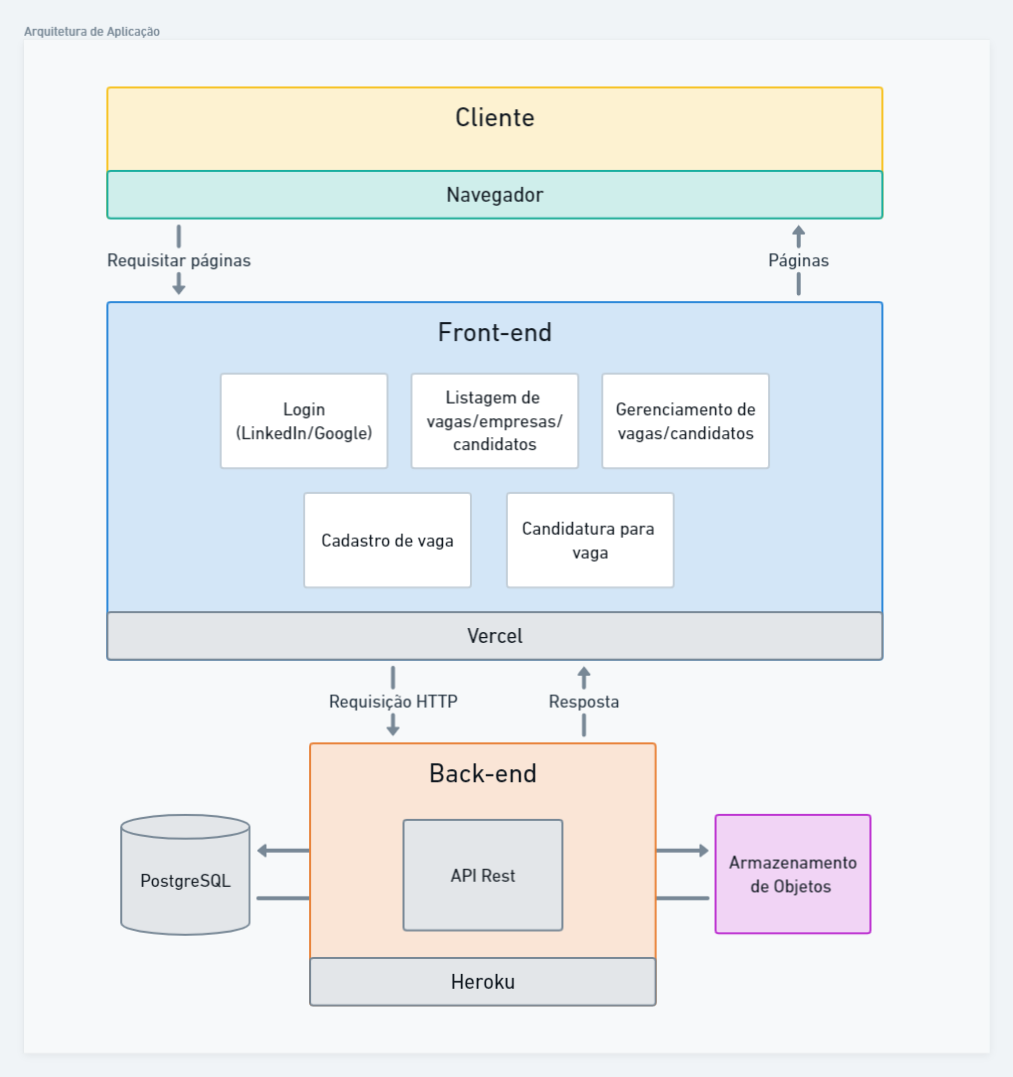
\includegraphics[width=0.95\textwidth]{imagens/arq-proj-arq-app2.png}
	\fonte{Produzido pelos autores utilizando a ferramenta \textit{Whimsical}}
\end{figure}

\begin{figure}[H]
	\centering
	\caption{\label{fig-arq-tec}Arquitetura Tecnológica}
	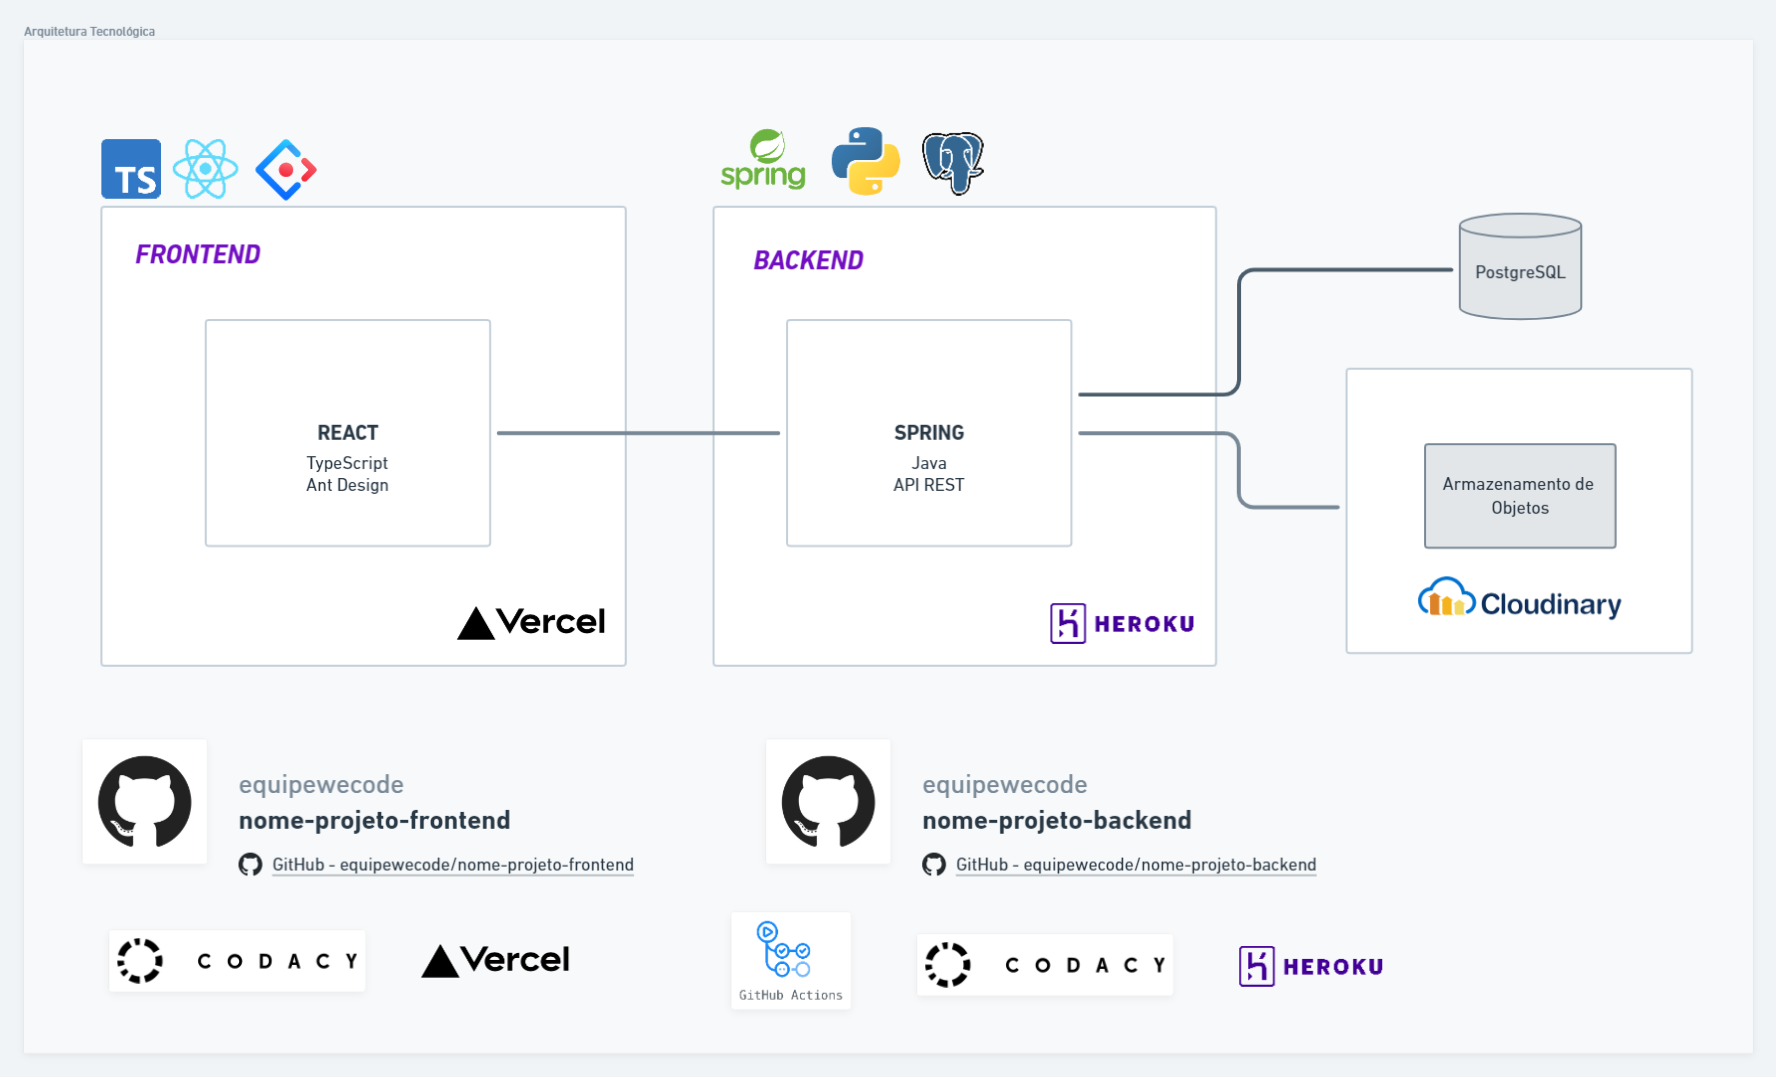
\includegraphics[width=0.95\textwidth]{imagens/arq-proj-arq-tec2.png}
	\fonte{Produzido pelos autores utilizando a ferramenta \textit{Whimsical}}
\end{figure}

\begin{figure}[H]
	\centering
	\caption{\label{fig-arq-negocio}Arquitetura de Negócios}
	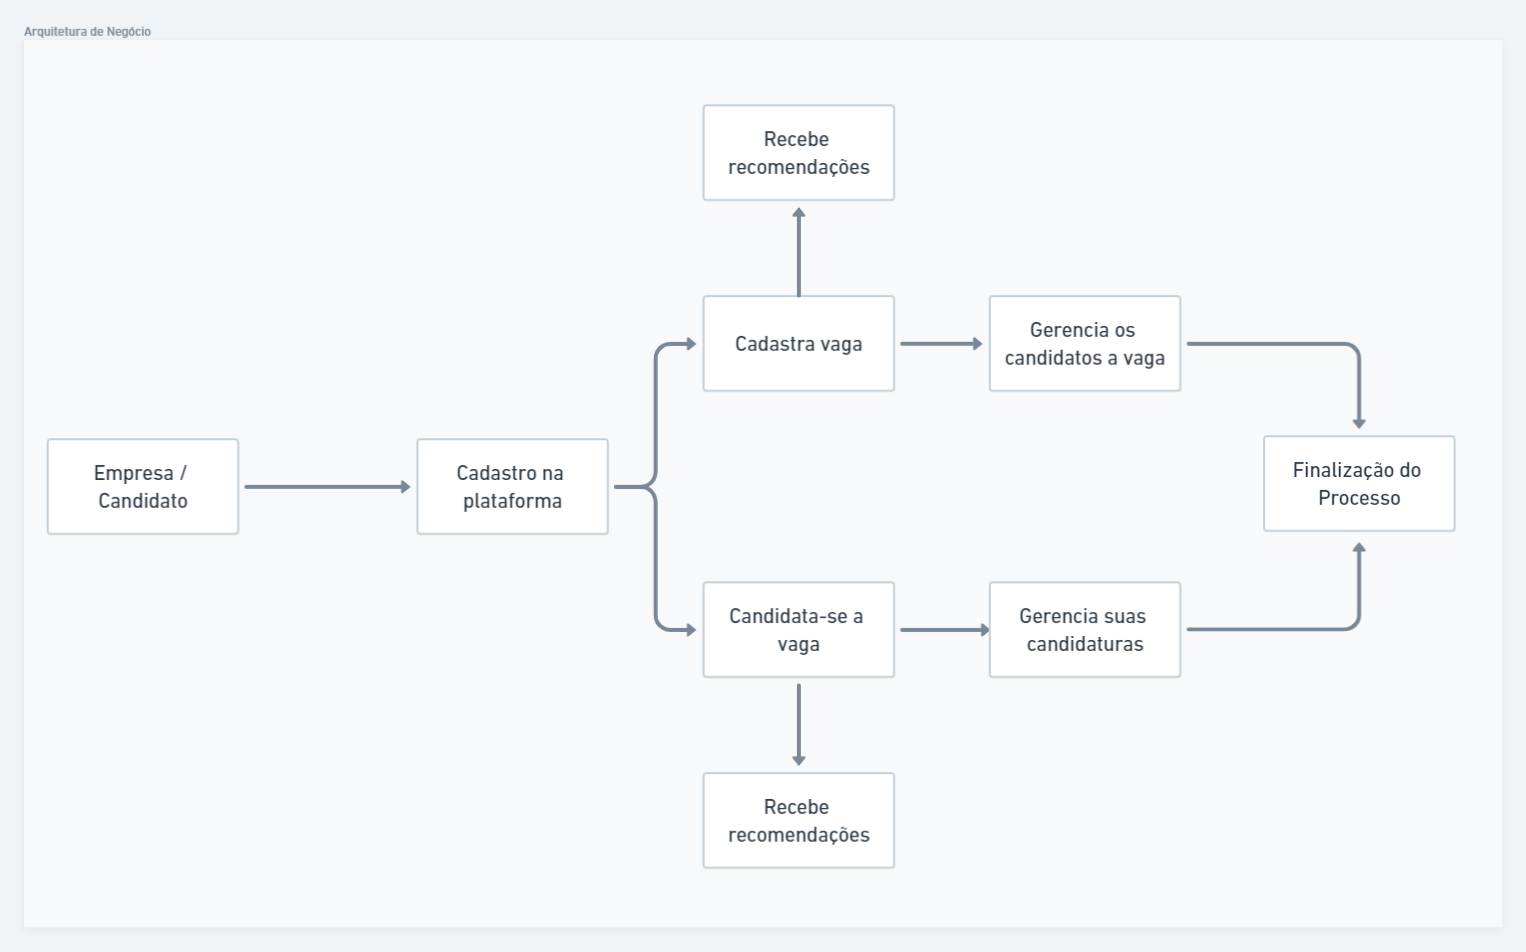
\includegraphics[width=0.95\textwidth]{imagens/arq-proj-arq-negocio2.png}
	\fonte{Produzido pelos autores utilizando a ferramenta \textit{Whimsical}}
\end{figure}